\usepackage[utf8]{inputenc}
\usepackage{slovak}
\usepackage{tikz}
\usepackage{fancybox}
\usepackage[english]{babel}
\uselanguage{English}
\languagepath{English}
\usetikzlibrary{arrows,positioning}
\usetheme{Warsaw}
\bibliographystyle{apalike}
\title{Sequential P Systems with Active Membranes Working on Sets}
\author{Michal Kováč}
\institute{FMFI UK, Slovakia}
\date{30.9.2015}
\begin{document}

\begin{frame}[t]
\titlepage
\end{frame}
\note{}

\section*{Outline}
\begin{frame}
\tableofcontents
\end{frame}
\note{}

\section{Overview of formal models} % (fold)
\label{sec:overview_of_formal_models}

  \subsection{P systems} % (fold)
  \label{sub:p_systems}

    \begin{frame}[t]\frametitle{Membrane structure}
      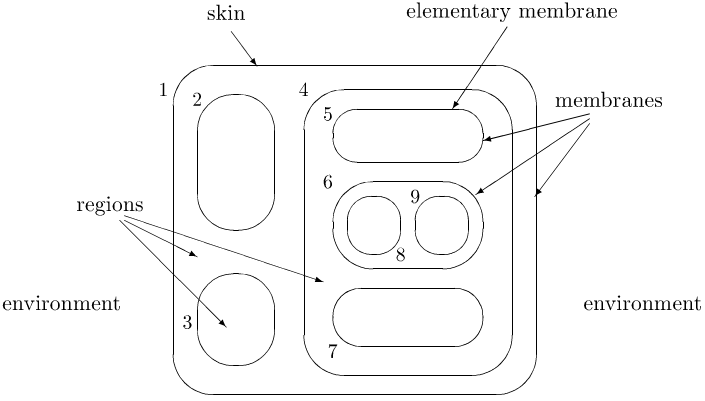
\includegraphics[width=0.7\textwidth]{membrane_structure.png}
      \hfill
      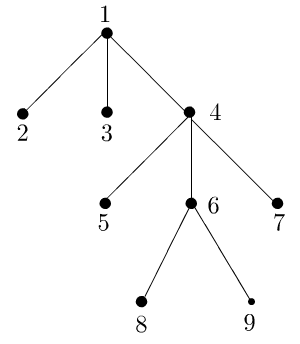
\includegraphics[width=0.3\textwidth]{membrane_tree.png}
      \pause
      \begin{itemize}
        \item Multisets
        \pause
        \item Rewriting rules
        \pause
        \item Passive vs. Active
      \end{itemize}

    \end{frame}
    \note{}

    \begin{frame}[t]\frametitle{P system with active membranes}
    \begin{itemize}
      \item $\Pi = (\Sigma, C_0, R_1, \ldots R_m)$
      \pause
      \item $C = (T, l, c)$
      \begin{itemize}
        \item $l: V(T) \rightarrow \{1, \ldots, m\}$
        \item $c: V(T) \rightarrow \mathbb{N}^\Sigma$
      \end{itemize}
      \pause
      \item Rewriting rules
      \begin{itemize}
        \item $u\rightarrow v$
        \item $u\rightarrow v\delta$
        \item $u\rightarrow [_j v]_j$,

        where $u \in \mathbb{N}^\Sigma, |u|\geq 1$ and $v\in \mathbb{N}^{\Sigma\times\{\cdot, \uparrow, \downarrow_{j}\}}$
      \end{itemize}

    \end{itemize}
    \end{frame}
    \note{}

    \begin{frame}[t]\frametitle{Computation}
      \begin{itemize}
        \item Maximal parallel vs. sequential
        \pause
        \item Language
        \begin{itemize}
          \item generating mode
          \item accepting mode
        \end{itemize}
      \end{itemize}

    \end{frame}
    \note{}

  % subsection p_systems (end)

  \subsection{Models with set semantics} % (fold)
  \label{sub:models_with_set_semantics}
    
    \begin{frame}[t]\frametitle{Multiset vs. set semantics}
      \begin{itemize}
        \item How realistic is the counting?
        \item Effectiveness of verification techniques
        \item No conflict (objects can participate as reactants in as many rules as they want)
      \end{itemize}
      
    \end{frame}
    \note{}

    \begin{frame}[t]\frametitle{Reaction systems}
      TODO: definition
    \end{frame}
    \note{}

    \begin{frame}[t]\frametitle{Set membane systems}
      \begin{itemize}
        \item Alhazov \cite{Alhazov05WithoutMultiplicities}: multiplicities of objects are ignored ~ R, with active membranes universal
        \item Kleijn, Koutny \cite{Kleijn11SetMembrane}: \"min-enabled\" computational step $\Rightarrow$ sequential ~ R
        \item maximal parallel $\Rightarrow$ deterministic
      \end{itemize}
    \end{frame}
    \note{}

  % subsection models_with_set_semantics (end)

% section overview_of_formal_models (end)

\section{Sequential active set membrane systems} % (fold)
\label{sec:sequential_active_set_membrane_systems}

  \subsection{Original semantics} % (fold)
  \label{sub:original_semantics}

    \begin{frame}[t]\frametitle{Sequential active set membrane systems}
      TODO: definition
    \end{frame}
    \note{}

    \begin{frame}[t]\frametitle{Proof of universality}
      TODO: proof of universality
    \end{frame}
    \note{}
  
  % subsection original_semantics (end)

  \subsection{inject-or-create semantics} % (fold)
  \label{sub:inject_or_create_semantics}

    \begin{frame}[t]\frametitle{inject-or-create}
      TODO: definition      
    \end{frame}
    \note{}

    \begin{frame}[t]\frametitle{inject-or-create}
      TODO: proof of universality
    \end{frame}
    \note{}

  % subsection inject_or_create_semantics (end)

  \subsection{wrap-or-create semantics} % (fold)
  \label{sub:wrap_or_create_semantics}
  
    \begin{frame}[t]\frametitle{wrap-or-create}
      TODO: definition
    \end{frame}
    \note{}

    \begin{frame}[t]\frametitle{wrap-or-create}
      TODO: proof of universality
    \end{frame}
    \note{}

  % subsection wrap_or_create_semantics (end)

% section sequential_active_set_membrane_systems (end)

\begin{frame}[plain]
  \bibliography{csp}
\end{frame}

\begin{frame}[plain]
  \begin{center}
    Thanks for your attention!
  \end{center}
\end{frame}

\end{document}
